\documentclass[14pt]{extbook}
\usepackage{multicol, enumerate, enumitem, hyperref, color, soul, setspace, parskip, fancyhdr} %General Packages
\usepackage{amssymb, amsthm, amsmath, bbm, latexsym, units, mathtools} %Math Packages
\everymath{\displaystyle} %All math in Display Style
% Packages with additional options
\usepackage[headsep=0.5cm,headheight=12pt, left=1 in,right= 1 in,top= 1 in,bottom= 1 in]{geometry}
\usepackage[usenames,dvipsnames]{xcolor}
\usepackage{dashrule}  % Package to use the command below to create lines between items
\newcommand{\litem}[1]{\item#1\hspace*{-1cm}\rule{\textwidth}{0.4pt}}
\pagestyle{fancy}
\lhead{Makeup Progress Quiz -1}
\chead{}
\rhead{Version B}
\lfoot{7547-2949}
\cfoot{}
\rfoot{Fall 2020}
\begin{document}

\begin{enumerate}
\litem{
Choose the graph of the equation below.\[ f(x) = - \sqrt[3]{x - 8} + 6 \]\begin{enumerate}[label=\Alph*.]
\begin{multicols}{2}\item 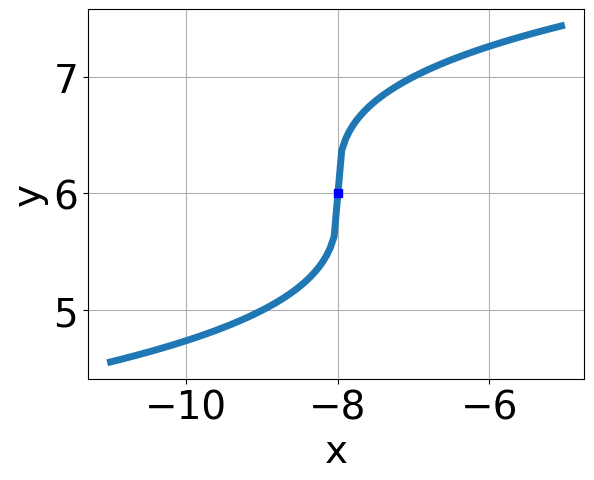
\includegraphics[width = 0.3\textwidth]{../Figures/radicalEquationToGraphCopyAB.png}\item 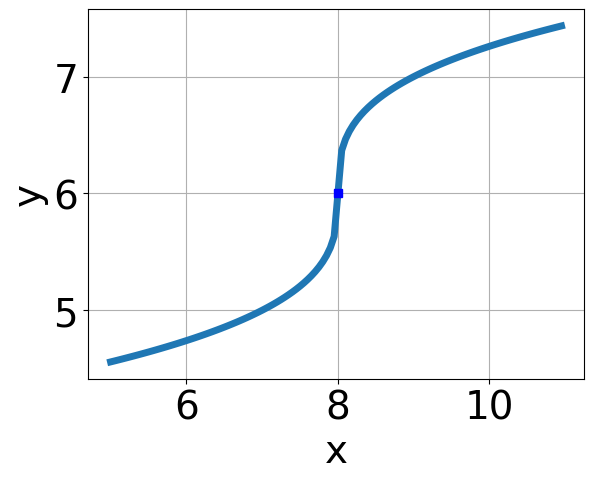
\includegraphics[width = 0.3\textwidth]{../Figures/radicalEquationToGraphCopyBB.png}\item 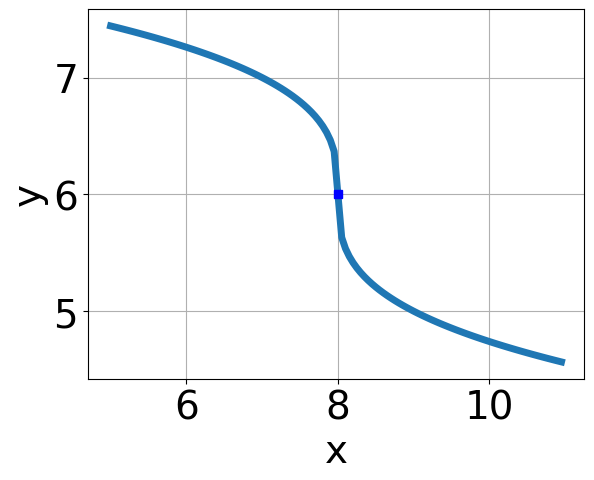
\includegraphics[width = 0.3\textwidth]{../Figures/radicalEquationToGraphCopyCB.png}\item 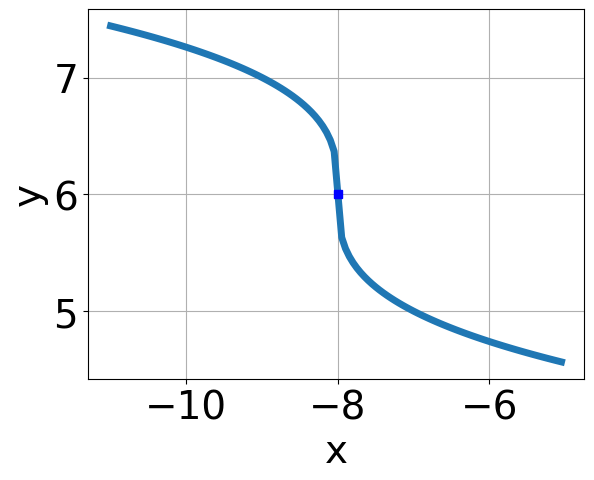
\includegraphics[width = 0.3\textwidth]{../Figures/radicalEquationToGraphCopyDB.png}\end{multicols}\item None of the above.
\end{enumerate} }
\litem{
Choose the graph of the equation below.\[ f(x) = \sqrt[3]{x + 14} - 7 \]\begin{enumerate}[label=\Alph*.]
\begin{multicols}{2}\item 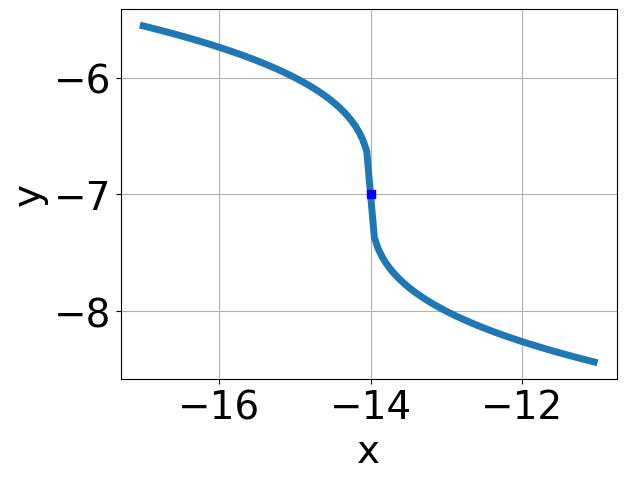
\includegraphics[width = 0.3\textwidth]{../Figures/radicalEquationToGraphAB.png}\item 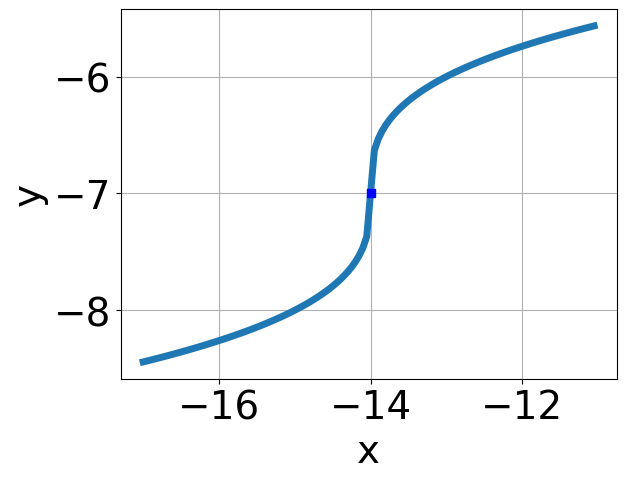
\includegraphics[width = 0.3\textwidth]{../Figures/radicalEquationToGraphBB.png}\item 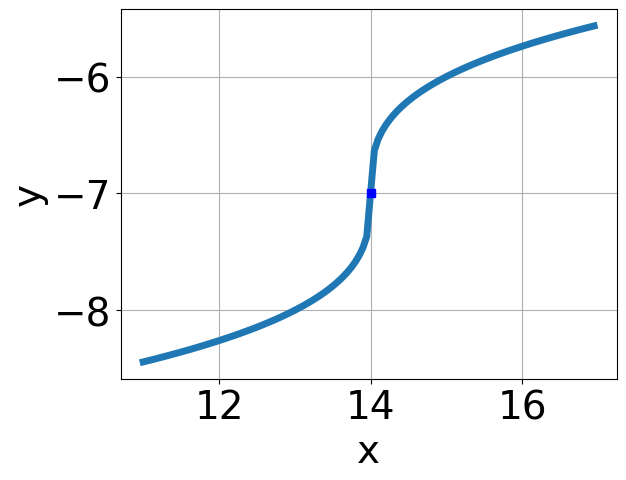
\includegraphics[width = 0.3\textwidth]{../Figures/radicalEquationToGraphCB.png}\item 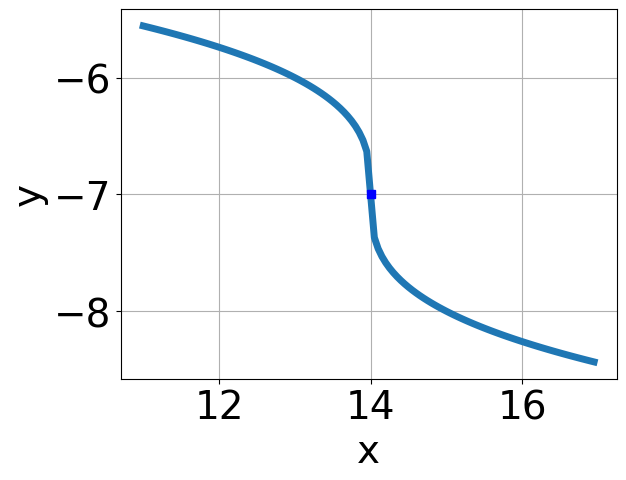
\includegraphics[width = 0.3\textwidth]{../Figures/radicalEquationToGraphDB.png}\end{multicols}\item None of the above.
\end{enumerate} }
\litem{
Solve the radical equation below. Then, choose the interval(s) that the solution(s) belongs to.\[ \sqrt{14 x^2 - 72} - \sqrt{-38 x} = 0 \]\begin{enumerate}[label=\Alph*.]
\item \( x_1 \in [-2.71, 5.29] \text{ and } x_2 \in [4,5] \)
\item \( x \in [-4,-1] \)
\item \( \text{All solutions lead to invalid or complex values in the equation.} \)
\item \( x \in [-2.71,5.29] \)
\item \( x_1 \in [-4, -1] \text{ and } x_2 \in [-2.71,2.29] \)

\end{enumerate} }
\litem{
Solve the radical equation below. Then, choose the interval(s) that the solution(s) belongs to.\[ \sqrt{8 x - 6} - \sqrt{-8 x - 4} = 0 \]\begin{enumerate}[label=\Alph*.]
\item \( x_1 \in [-0.96, -0.29] \text{ and } x_2 \in [-0.25,5.75] \)
\item \( \text{All solutions lead to invalid or complex values in the equation.} \)
\item \( x \in [0.48,0.65] \)
\item \( x_1 \in [-0.43, 0.17] \text{ and } x_2 \in [-0.25,5.75] \)
\item \( x \in [-0.43,0.17] \)

\end{enumerate} }
\litem{
Choose the equation of the function graphed below.
\begin{center}
    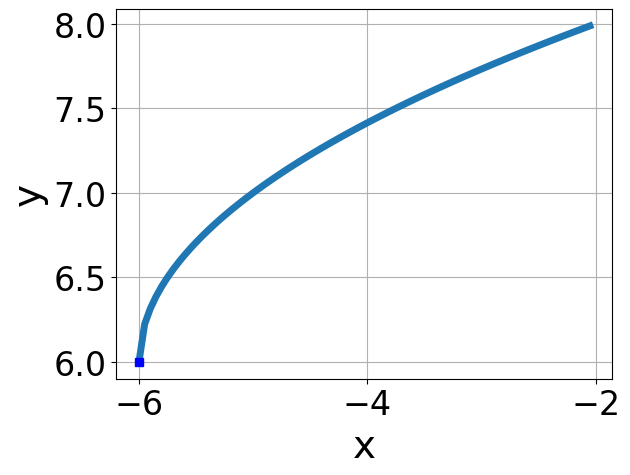
\includegraphics[width=0.5\textwidth]{../Figures/radicalGraphToEquationB.png}
\end{center}
\begin{enumerate}[label=\Alph*.]
\item \( f(x) = \sqrt{x + 6} + 6 \)
\item \( f(x) = \sqrt{x - 6} + 6 \)
\item \( f(x) = - \sqrt{x - 6} + 6 \)
\item \( f(x) = - \sqrt{x + 6} + 6 \)
\item \( \text{None of the above} \)

\end{enumerate} }
\litem{
What is the domain of the function below?\[ f(x) = \sqrt[7]{-6 x + 8} \]\begin{enumerate}[label=\Alph*.]
\item \( \text{The domain is } (-\infty, a], \text{   where } a \in [0.99, 1.37] \)
\item \( \text{The domain is } [a, \infty), \text{   where } a \in [0.85, 1.64] \)
\item \( (-\infty, \infty) \)
\item \( \text{The domain is } [a, \infty), \text{   where } a \in [0.71, 1.21] \)
\item \( \text{The domain is } (-\infty, a], \text{   where } a \in [0.49, 1.26] \)

\end{enumerate} }
\litem{
Choose the equation of the function graphed below.
\begin{center}
    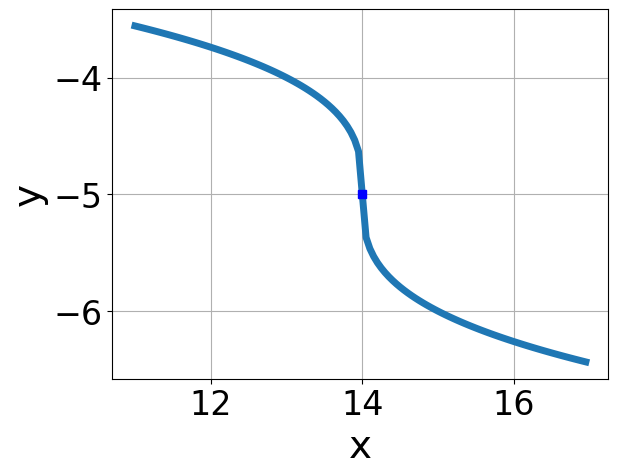
\includegraphics[width=0.5\textwidth]{../Figures/radicalGraphToEquationCopyB.png}
\end{center}
\begin{enumerate}[label=\Alph*.]
\item \( f(x) = - \sqrt[3]{x + 14} - 5 \)
\item \( f(x) = - \sqrt[3]{x - 14} - 5 \)
\item \( f(x) = \sqrt[3]{x - 14} - 5 \)
\item \( f(x) = \sqrt[3]{x + 14} - 5 \)
\item \( \text{None of the above} \)

\end{enumerate} }
\litem{
What is the domain of the function below?\[ f(x) = \sqrt[5]{4 x - 8} \]\begin{enumerate}[label=\Alph*.]
\item \( \text{The domain is } (-\infty, a], \text{   where } a \in [-2.3, 1.1] \)
\item \( \text{The domain is } [a, \infty), \text{   where } a \in [0.46, 1.57] \)
\item \( \text{The domain is } (-\infty, a], \text{   where } a \in [1.2, 2.1] \)
\item \( (-\infty, \infty) \)
\item \( \text{The domain is } [a, \infty), \text{   where } a \in [0.72, 3.83] \)

\end{enumerate} }
\litem{
Solve the radical equation below. Then, choose the interval(s) that the solution(s) belongs to.\[ \sqrt{12 x^2 + 14} - \sqrt{-34 x} = 0 \]\begin{enumerate}[label=\Alph*.]
\item \( x \in [-0.92,-0.49] \)
\item \( \text{All solutions lead to invalid or complex values in the equation.} \)
\item \( x \in [-3.06,-1.82] \)
\item \( x_1 \in [-0.27, 0.9] \text{ and } x_2 \in [1.33,4.33] \)
\item \( x_1 \in [-3.06, -1.82] \text{ and } x_2 \in [-1.5,0.5] \)

\end{enumerate} }
\litem{
Solve the radical equation below. Then, choose the interval(s) that the solution(s) belongs to.\[ \sqrt{-3 x - 2} - \sqrt{4 x + 6} = 0 \]\begin{enumerate}[label=\Alph*.]
\item \( x \in [-0.09,2.26] \)
\item \( x \in [-1.25,-0.58] \)
\item \( x_1 \in [-1.88, -1.2] \text{ and } x_2 \in [-2.67,3.33] \)
\item \( \text{All solutions lead to invalid or complex values in the equation.} \)
\item \( x_1 \in [-1.25, -0.58] \text{ and } x_2 \in [-2.67,3.33] \)

\end{enumerate} }
\end{enumerate}

\end{document}